\chapter{OmniTools}\label{AppendiceC}

在章節 \ref{chap:HIP Tools} 中,我們介紹了來自 ROCm 堆疊中的強大工具 rocTracer 和 rocProfiler。這些工具提供了在 HIP 程式執行過程中收集效能資料的基本功能。然而,儘管這些工具能夠收集原始效能指標,但它們提供的分析能力有限。

為了彌補這個缺點並提供一套更完整的效能分析工具,AMD 開發了 Omnitrace 和 Omniperf。需要注意的是,這些工具沒有包含在 ROCm 堆疊的標準套件內,而是 AMD 所發起的研究專案,目的是為社群提供更先進的工具選擇。因此,我們並未在章節 \ref{chap:HIP Tools} 中討論這些工具,而是在本附錄章節中介紹這些強大的工具。

從高層次來看,Omnitrace 和 Omniperf 都有助於效能分析。Omnitrace 提供了 CPU 和 GPU 執行的追蹤,幫助使用者了解執行模式並找出潛在的效能瓶頸。而 Omniperf 則深入分析 GPU 核心的效能,評估硬體的利用情況。使用者應該先使用 Omnitrace 來識別有問題的核心,然後再使用 Omniperf 進一步深入了解核心效能的問題。


\section{Omnitrace}
Omnitrace 是由 AMD Research 開發的開源專案,為了協助分析執行於 AMD 異構系統上的軟體效能而設計。Omnitrace 可以針對多種程式語言(如 C、C++、Fortran、HIP、OpenCL 和 Python)進行效能剖析與追蹤。它提供多種功能,包含二進位檔案插樁 (binary instrumentation)(僅支援 CPU)與呼叫堆疊採樣 (call-stack sampling),以收集追蹤資料來支援效能分析。這些追蹤資料可以用於互動式的視覺化,或用於生成高層次的效能剖析報告。

在本書中,我們將略過這些工具的安裝過程,因為相關指引可以在 Omnitrace 的開源專案網站 \url{https://github.com/ROCm/Omnitrace} 中找到。更詳盡的文件也可以參考 \url{https://amdresearch.github.io/Omnitrace/} 網站。

\subsection{Omnitrace 配置檔案}
Omnitrace 配置檔案決定了 Omnitrace 命令列工具的預設行為。這個配置檔案可以透過使用以下指令,使用命令列工具 \lstinline|omnitrace-avail| 來生成:

\lstinline|omnitrace-avail -G ./omnitrace.cfg|

生成的檔案應該是自我文件化 (self-documented) 的。如果我們需要更詳細的選項說明,可以使用 \lstinline|--all| 參數。我們可以將此參數加到指令中,以輸出額外的資訊,提供更多細節。若要使用配置檔案,應將其路徑加入 \lstinline|OMNITRACE_CONFIG_FILE| 環境變數中。


\subsection{收集追蹤資料}
Omnitrace 提供兩種追蹤收集方法:1) 呼叫堆疊採樣 (call-stack sampling) 與 2) 二進位檔案插樁 (binary instrumentation)。選擇哪一種方法取決於使用者的需求。呼叫堆疊採樣適合用來收集所有函數的追蹤資料(參見圖 \ref{fig:call-stack-sampling})。相較之下,二進位檔案插樁則是針對特定函數進行追蹤,因為這樣可以減少追蹤的開銷和追蹤資料的大小,並提供更精確的效能剖析結果(參見圖 \ref{fig:binary-instrumentation})。除了這些差異,這兩種方法也可以一起使用,透過呼叫堆疊採樣來記錄所有函數的追蹤資料,同時使用二進位檔案插樁為特定函數提供高精度的時間戳記錄。

\begin{figure}
    \centering
    \begin{subfigure}[b]{\textwidth}
        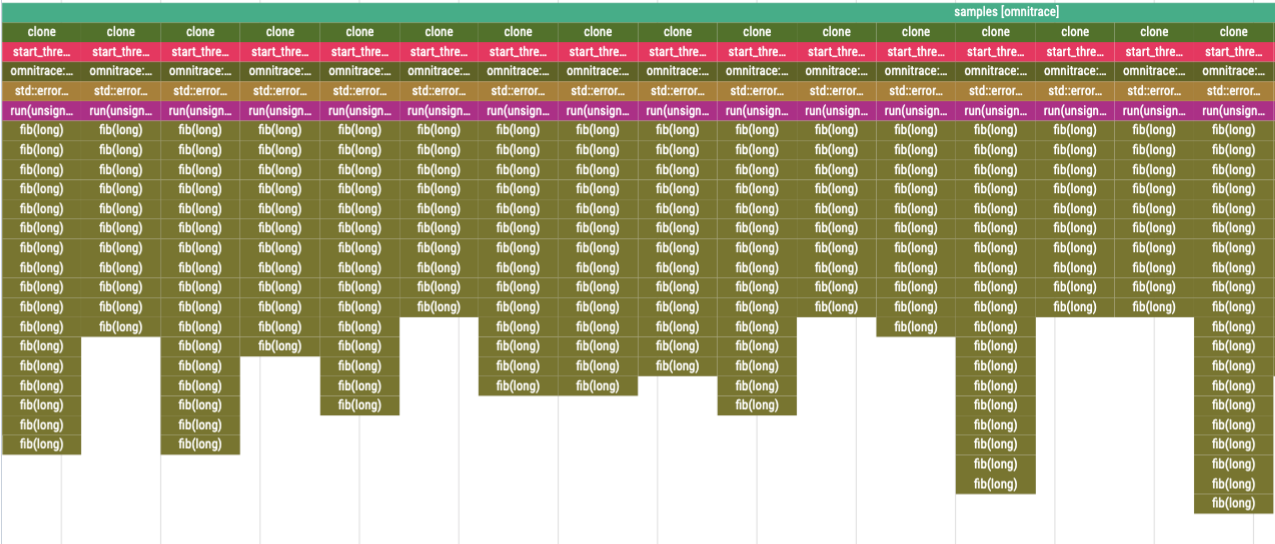
\includegraphics[width=\linewidth]{Appendici/CallStackSampling.png}
        \caption{呼叫堆疊採樣 (call-stack sampling)}
        \label{fig:call-stack-sampling}
    \end{subfigure}

    \begin{subfigure}[b]{\textwidth}
        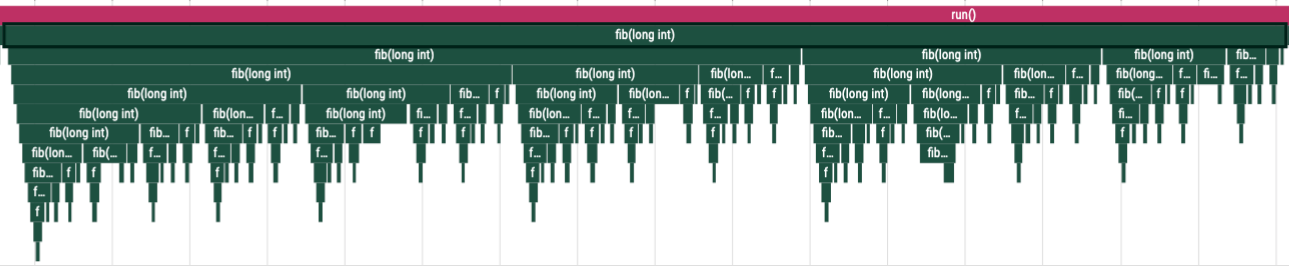
\includegraphics[width=\linewidth]{Appendici/BinaryInstrumentation.png}
        \caption{二進位檔案插樁 (binary instrumentation)}
        \label{fig:binary-instrumentation}
    \end{subfigure}

    \caption{比較使用呼叫堆疊採樣 (call-stack sampling) 和二進位檔案插樁 (binary instrumentation) 在執行遞迴斐波那契數計算程式時所產生的追蹤資料。\\呼叫堆疊採樣方法的解析度有限,無法捕捉精確的函數開始和結束時間。}
    
\end{figure}


無論選擇哪種方法,建議使用者在編譯執行檔時啟用優化 (\lstinline|-O2| 或更高)、禁用 assertion (\lstinline|-DNDEBUG|),並包含除錯資訊(指定 \lstinline|-g1| 或更高的級別)。

\paragraph{呼叫堆疊採樣 (call-stack sampling)}
呼叫堆疊採樣可以透過執行 \lstinline|omnitrace-sample| 執行檔來啟動。例如,如果要執行的 GPU 程式叫做 \lstinline|foo|,以下指令會使用呼叫堆疊採樣來執行 foo:

\lstinline|omnitrace-sample -- foo|

\lstinline|omnitrace-sample| 執行檔使用一般的 LLM 風格命令列參數語法。所有雙連字號 \lstinline|--| 前的參數是給 Omnitrace 的,而 \lstinline|--| 後面的參數則是給程式的。

\paragraph{二進位檔案插樁 (binary instrumentation)}
二進位檔案插樁可以透過執行 \lstinline|omnitrace-instrument| 執行檔來完成,該工具會修改主程式,插入收集追蹤的程式碼。預設情況下,\lstinline|omnitrace-instrument| 會同時插樁並執行程式。其語法與 \lstinline|omnitrace-sample| 類似,\lstinline|omnitrace-instrument| 的參數和程式的參數由雙連字號 \lstinline|--| 分開。

另外,\lstinline|omnitrace-instrument| 也可以連接到正在運行的程序,或者生成已插樁的二進位檔案以供稍後執行。若要連接到正在運行的程序,請使用 \lstinline|-p| 參數,後面跟著程序 ID(PID),如以下指令所示:

\lstinline|omnitrace-instrument <omnitrace-options> -p <PID> -- <exe-name>|

若要創建已插樁的二進位檔案,請使用 \lstinline|-o| 參數來指定輸出的檔案名稱,如以下指令所示:

\lstinline|omnitrace-instrument <omnitrace-options> -o <name-of-new-exe-or-library> -- <exe-or-library>|

如同讀者可能已經注意到,我們並未指定要為哪些函數來收集追蹤資料。這是因為 Omnitrace 有一個預設規則來選擇要插樁的函數。預設情況下,所有函數都會被插樁追蹤,除非函數符合以下條件:1) 動態呼叫位址(例如函數指標),或 2) 少於 1024 個指令。\footnote{有更多規則會防止函數被插樁。請參閱 Omnitrace 文件以獲得更多資訊。}

\lstinline|omnitrace-instrument| 工具提供了三組參數來自訂要插樁的模組(函式庫)與函數。\lstinline|--module-include| 和 \lstinline|--function-include| 參數分別允許使用者加入預設插樁規則以外的模組和函數。這些參數可以使用正規表達式來匹配模組和函數名稱。相對地,\lstinline|--module-restrict| 和 \lstinline|--function-restrict| 參數則會覆寫預設的選擇,只包含與提供的正規表達式匹配的模組和函數。最後,\lstinline|--module-exclude| 和 \lstinline|--function-exclude| 參數讓使用者能夠調整選擇,將一些預設的模組和函數排除。

\subsection{輸出與視覺化}
Omnitrace 的輸出會儲存於以下路徑:

\lstinline|<OUTPUT_PATH>[/<TIMESTAMP>]/[<PREFIX>]<DATA_NAME>[<OUTPUT_SUFFIX>].<EXT>|

透過設定一些環境變數,我們可以指定資料追蹤的輸出位置與檔案名稱。例如,\lstinline|OMNITRACE_OUTPUT_PATH| 環境變數可以用來指定儲存輸出檔案目錄的路徑。在路徑中,使用者可以插入特殊的佔位符號來描述追蹤資料的內容。這些佔位符號包括 \lstinline|%argt%|、\lstinline|%ppid%|、\lstinline|%pid%| 和 \lstinline|%rank%|,分別代表執行檔的 basename、父程序 ID、程序 ID 和 MPI rank。若要查看完整的選項列表,包含其描述,使用者可以執行指令 \lstinline|omnitrace-avail –list-keys –expand-keys|

每次執行 Omnitrace 時,會生成一個 \lstinline|perfetto-trace.proto| 的檔案。該檔案可以透過 Perfetto 視覺化工具來開啟,該工具可於以下網址取得:\url{ui.perfetto.dev}(參見圖 \ref{fig:omnitrace-visualization} 查看範例)

\begin{figure}
    \centering
    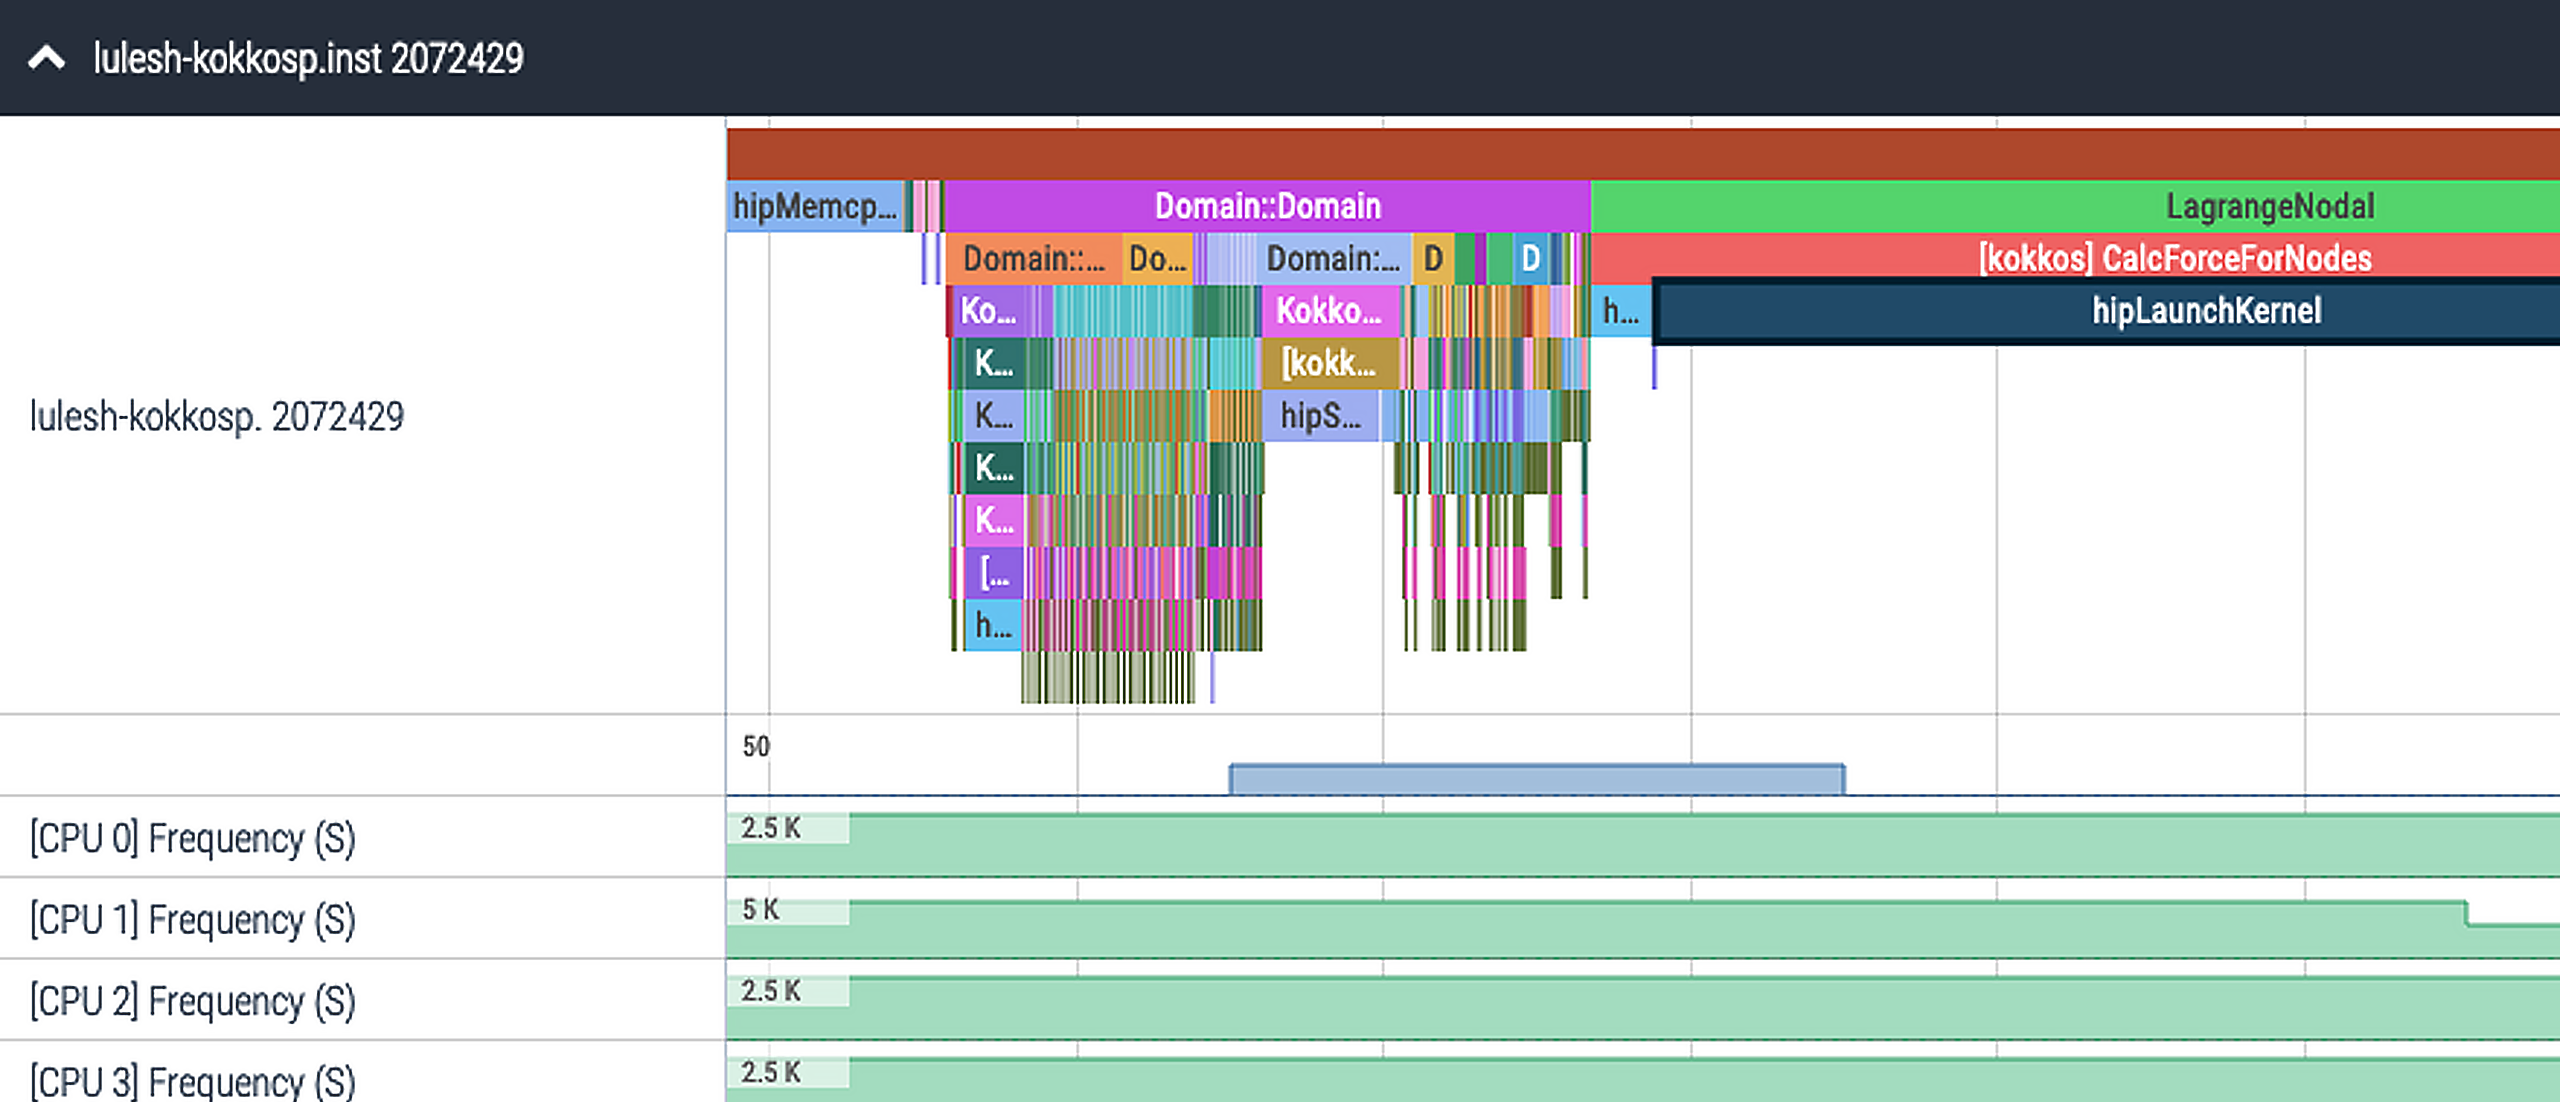
\includegraphics[width=1\linewidth]{Appendici/OmnitraceVisualization.png}
    \caption{使用 Omnitrace 生成的追蹤資料視覺化的範例}
    \label{fig:omnitrace-visualization}
\end{figure}


\section{Omniperf}

相對於專注於主機端函數呼叫剖析的 Omnitrace,Omniperf 提供了 kernel 層級的剖析功能。Omniperf 基於 rocProf 開發,能夠對在 AMD Instinct MI GPU(例如 MI100、MI200 和 MI300 系列 GPU)上運行的機器學習(ML)和高效能運算(HPC)的工作進行剖析。

Omniperf 擁有全面的功能,提供各種面板來做深入的分析,包括 System Speed-of-Ligh 與  Memory Chart Analysis。該工具同時支援命令列和圖形使用者介面(GUI)分析,以滿足不同使用者的需求,並增強對效能資料的整體取得能力。


\subsection{使用 Omniperf 剖析程式}
Omniperf 的核心是一個可以以剖析模式啟動程式的命令列工具。假設我們的 GPU 程式名為 \lstinline|vcopy|,以下指令可以收集程式中所有 kernel 的所有可用計數器:

\lstinline|omniperf profile -n vcopy_data -- ./vcopy -n 1048576 -b 256|

與 Omnitrace 類似,雙連字號 \lstinline|--|用來分隔 Omniperf 的參數和我們想要剖析的程式名稱。Omniperf 的 \lstinline|-n| 參數定義了輸出的目錄名稱。在這個例子中,輸出將會儲存在目錄 \lstinline|./workloads/vcopy_data/MI200| 中。值得注意的是,除非使用 \lstinline|-p|/\lstinline|--path| 參數來覆寫輸出路徑,Omniperf 會將加速器的名稱附加為目錄的最後一層。

收集所有 kernel 的追蹤資料是非常耗時的。由於硬體效能計數器的數量有限,通常需要多次重新執行 kernel 才能收集所有的指標。為了減少收集特定指標的執行時間,Omniperf 提供了幾個參數,包括:

\begin{itemize}
\item \lstinline|-k|/\lstinline|--kernel| 可以根據 kernel 的名稱過濾 kernel。
\item \lstinline|-d|/\lstinline|--dispatch| 可以根據派遣 ID(即第 n 個派遣的 kernel)過濾 kernel。
\item \lstinline|-b|/\lstinline|--block| 可以根據硬體元件區塊 (hardware component blocks) 過濾指標。
\end{itemize}

除了除錯典型的效能瓶頸外,Omniperf 還可以用來生成用來做 roofline 分析的指標 \cite{williams2009roofline}。如果不需要收集 roofline 分析的指標,可以透過指定 \lstinline|--no-roof| 來讓 Omniperf 執行而不收集相關的剖析資料。或者,我們也可以選擇加入 \lstinline|--roof-only| 參數來只剖析 roofline 分析的指標。

使用 empirical roofline model, 使用者可以視覺化比較應用程式的實際效能與機器的最大可達效能。Omniperf 的 roofline 分析功能會直接生成 roofline 視覺化圖表,並以 PDF 格式輸出(請參見圖 \ref{fig:roofline1} 和圖 \ref{fig:roofline2})。

\begin{figure}
    \centering
    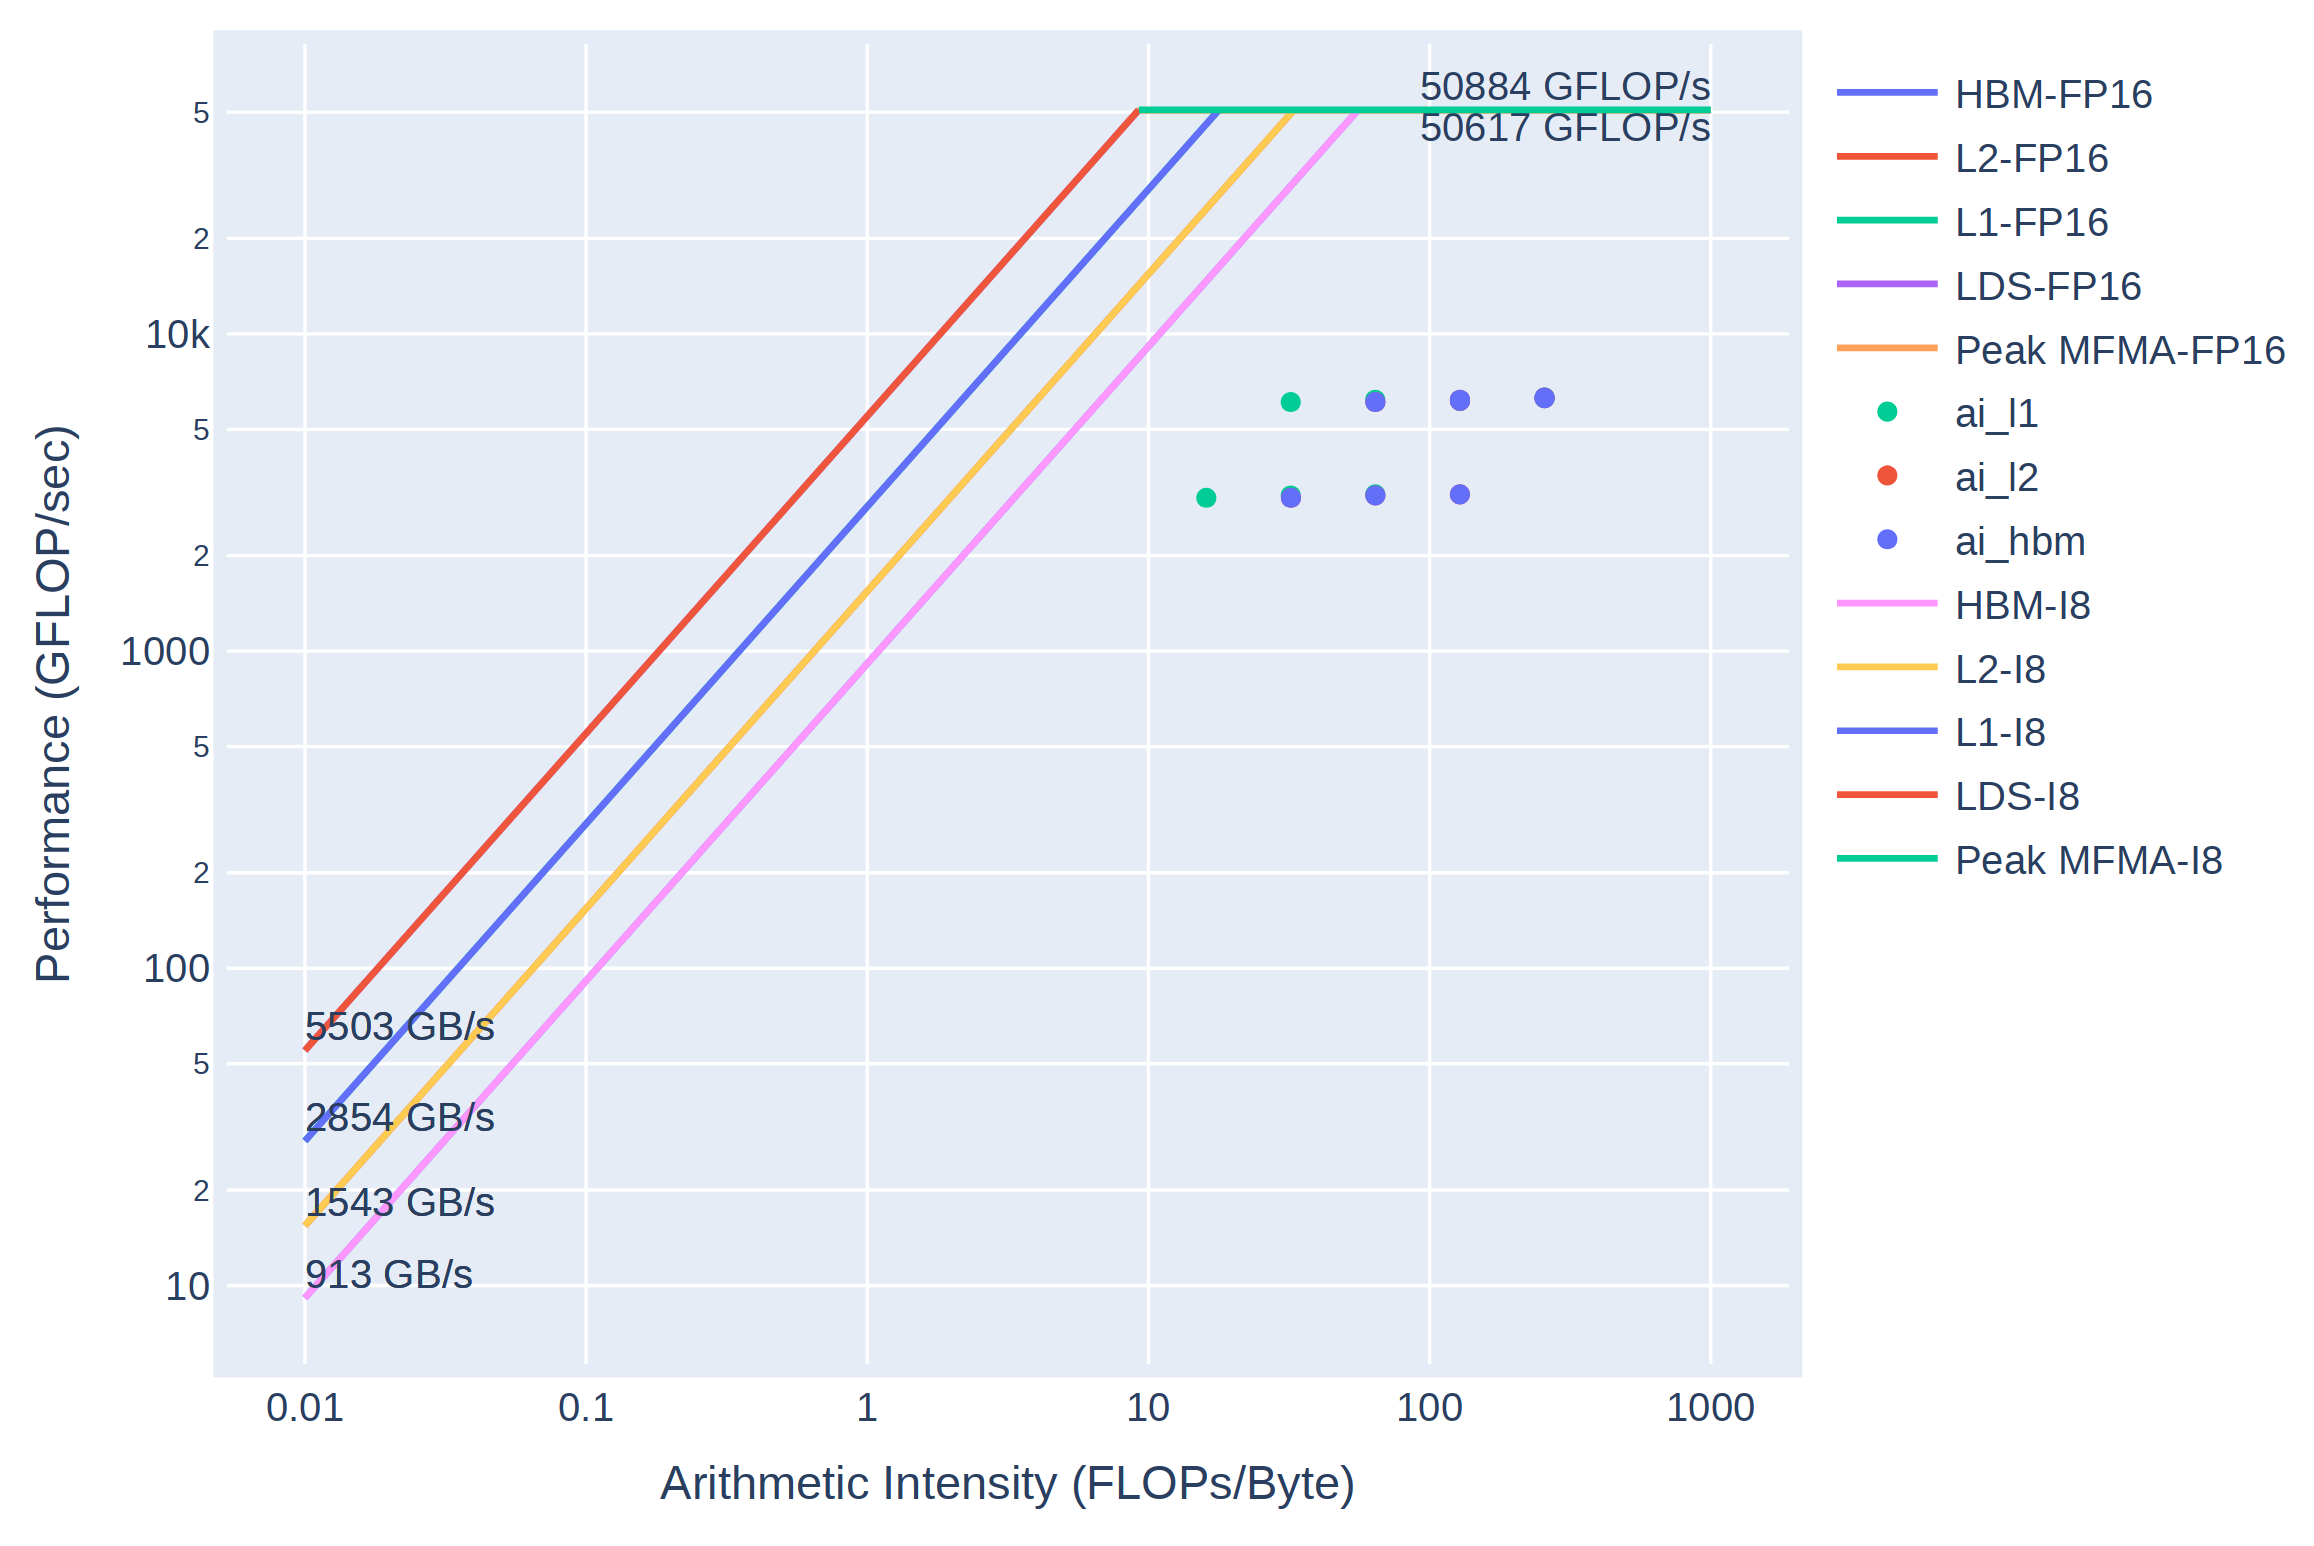
\includegraphics[width=1\linewidth]{Appendici/Roofline1.png}
    \caption{8 位元整數與 16 位元浮點運算的 roofline 分析圖表}
    \label{fig:roofline1}
\end{figure}

\begin{figure}
    \centering
    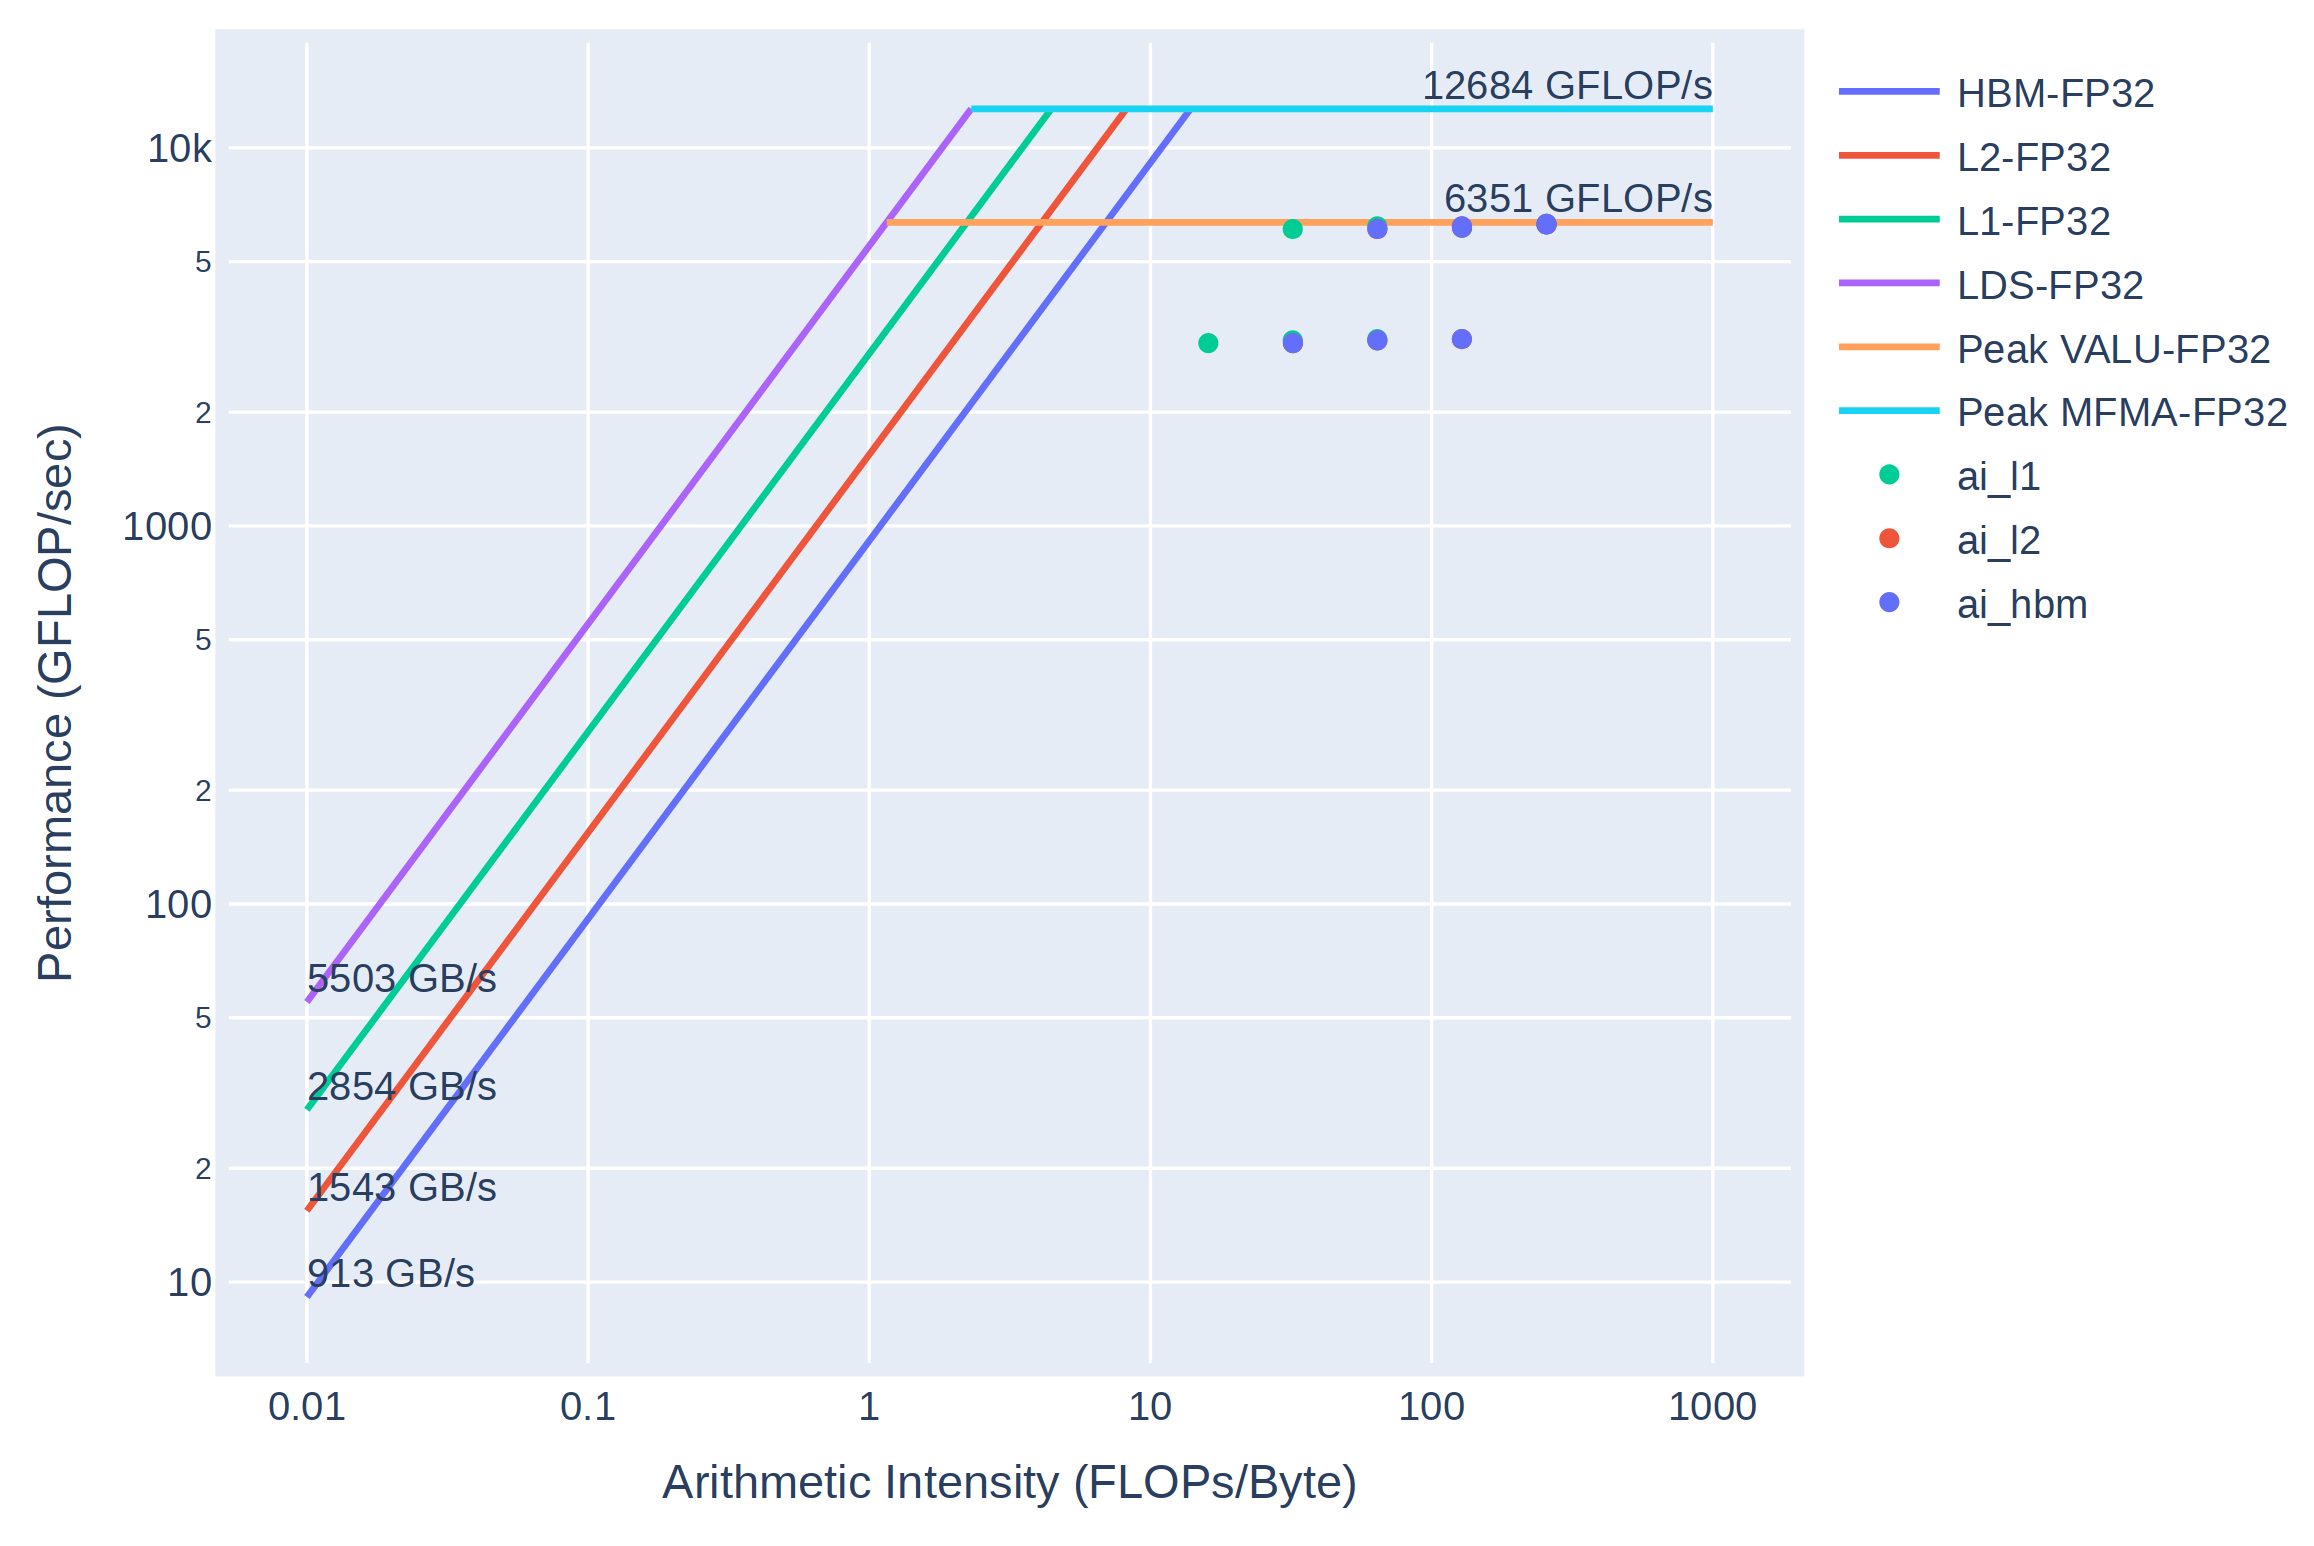
\includegraphics[width=1\linewidth]{Appendici/Roofline2.png}
    \caption{32 位元整數與 64 位元浮點運算的 roofline 分析圖表}
    \label{fig:roofline2}
\end{figure}

\subsection{使用命令列介面進行分析}
收集的原始剖析資料對大多數使用者來說不容易解讀。為了解決這個問題,Omniperf 提供了一個分析工具,該工具會處理資料來簡化詮釋的過程。這個分析工具也內建於 \lstinline|omniperf| 命令列工具中。我們可以使用以下指令來啟動此工具:

\lstinline|omniperf analyze -p workloads/vcopy/MI200/|

在這裡,參數 \lstinline|-p| 需要提供在剖析階段時收集的原始指標的路徑。

分析工具會將處理後的資料以表格形式顯示在命令列介面中(參見圖 \ref{fig:omniperf-cli})。輸出通常包含三個部分,包含高層次的狀態資訊(kernel 與其執行時間)、系統資訊以及系統的 Speed-of-
Light 分析(即衍生的效能指標)。衍生的效能指標的意義通常是能夠自我解釋的,但使用者仍然可以參考 Omniperf 文件來獲得更詳細的解釋。\footnote{\url{https://rocm.github.io/omniperf/performance_model.html}}

此外,Omniperf 的命令列介面分析工具也支援比較兩次不同的執行結果。假設原始剖析輸出儲存在 \lstinline|workload1/path| 和 \lstinline|workload2/path|,我們可以使用以下指令來比較它們:

\lstinline|omniperf analyze -p workload1/path -p workload2/path|

Omniperf 的分析工具可以並排顯示衍生的效能指標,以方便比較(參見圖 \ref{fig:omniperf-compare})。

\begin{figure}
    \centering
    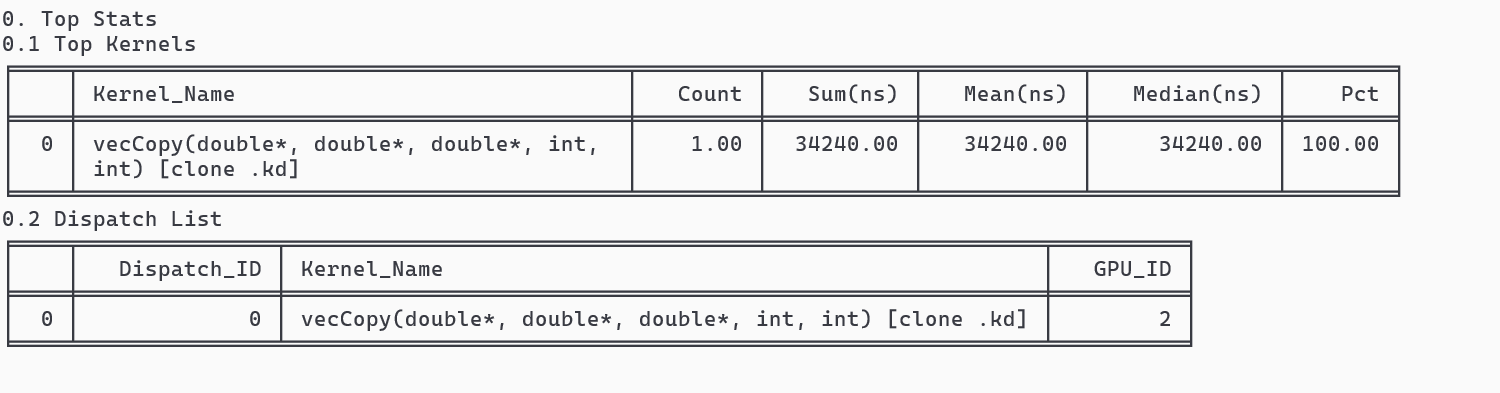
\includegraphics[width=1\linewidth]{Appendici/OmniperfCLI.png}
    \caption{命令列介面分析工具輸出的開始部分}
    \label{fig:omniperf-cli}
\end{figure}

\begin{figure}
    \centering
    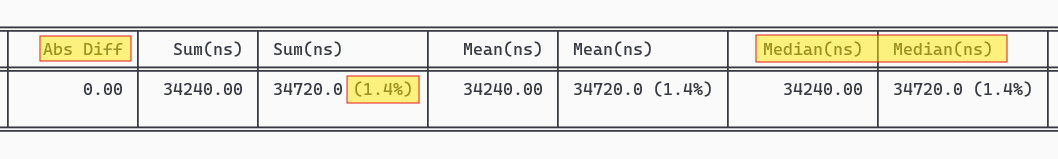
\includegraphics[width=1\linewidth]{Appendici/OmniperfCompare.png}
    \caption{Omniperf 分析工具在比較兩次執行時的輸出。Count、Sum、Mean 和 Median 等欄位會顯示兩次,第二次顯示的是 workload 2 的資料。相對差異也會顯示在 workload 2 的欄位中。}
    \label{fig:omniperf-compare}
\end{figure}


\subsection{使用網頁 GUI 進行分析}
為了提供更使用者友善的效能分析介面,Omniperf 可以啟動一個基於 Flask \cite{grinberg2018flask} 的網頁伺服器。使用者可以透過網頁瀏覽器來檢視結果。只需要在 \lstinline|omniperf analyze| 指令中加入 \lstinline|--gui| 參數,如下指令所示:

\lstinline|omniperf analyze -p workloads/vcopy/MI200 --gui|

開啟網頁介面的 URL 會顯示在終端機中(如 \url{http://127.0.0.1:8050})。預設情況下,Omniperf 使用 8050 連接埠。

網頁介面(參見圖 \ref{fig:omniperf-web-interface})包括一個控制面板(上方)、記憶體分析面板(中間)和 roofline 分析面板(底部)。使用者可以使用下拉選單來過濾分析結果,選擇特定的 kernel 與要關注的 kernel dispatch。

\begin{figure}
    \centering
    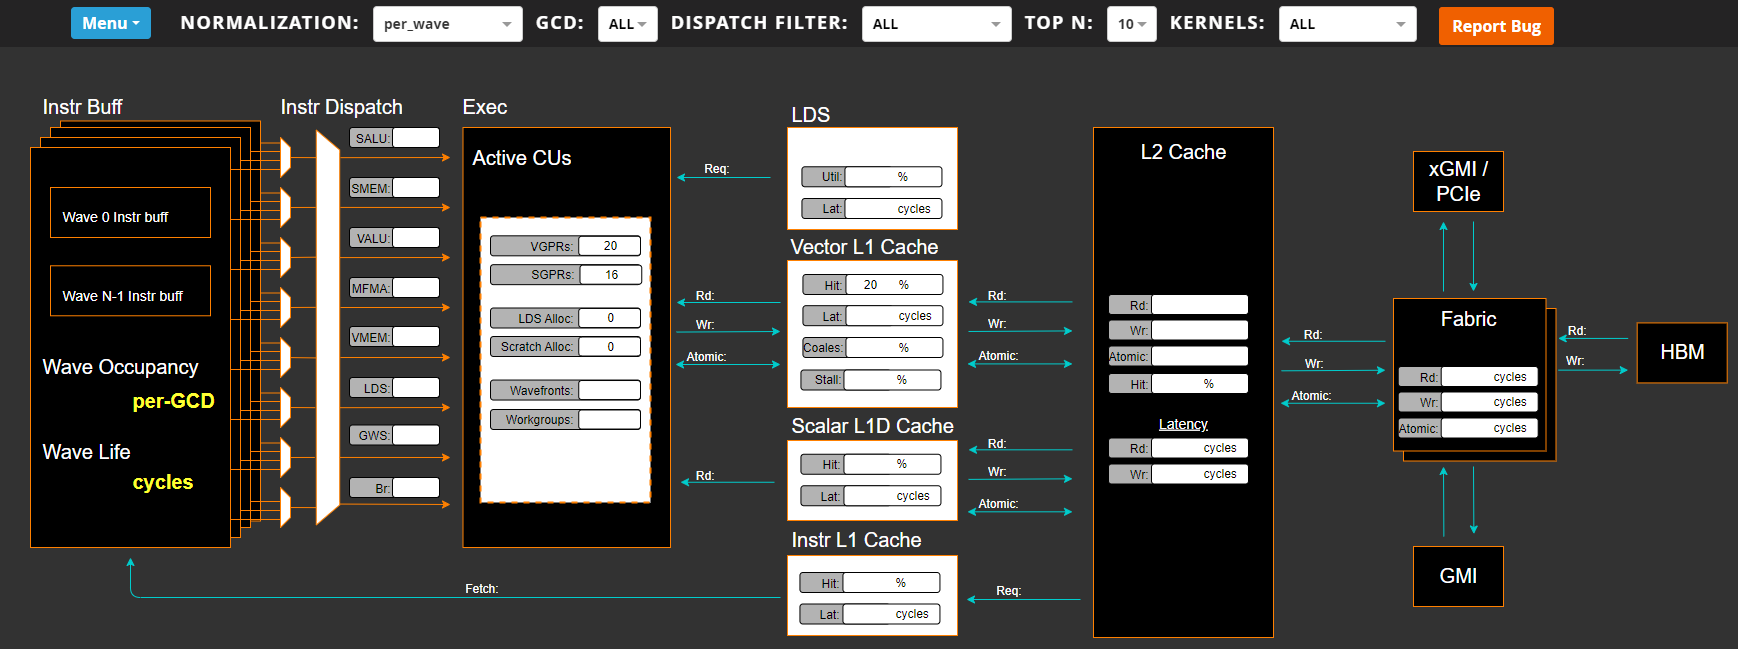
\includegraphics[width=1\linewidth]{Appendici/OmniperfWebInterface.png}
    \caption{基於網頁的 Omniperf 分析 GUI 介面}
    \label{fig:omniperf-web-interface}
\end{figure}


\subsection{使用 Grafana 進行分析}
儘管簡單的網頁 GUI 提供了更具使用者友善的效能分析介面,但呈現的資料仍然有限。為了進行全面的 GUI 基礎效能分析,Omniperf 使用了 Grafana \cite{chakraborty2021grafana},一個受歡迎的資料視覺化框架。Grafana 需要將資料儲存於 MongoDB 資料庫中。因此,Omniperf 提供了一個工具,可以使用以下命令將原始指標匯入 MongoDB 資料庫:

\lstinline|omniperf database --import -H 127.0.0.1 -u temp -t asw -w workloads/vcopy/mi200|

這邊的參數 \lstinline|-H| 和 \lstinline|-u| 分別接受 MongoDB 實例的主機 IP 位址與使用者名稱。\lstinline|-t|(team)和 \lstinline|-w|(workload)是用來決定資料庫名稱的參數。預設情況下,資料庫名稱為:

\lstinline|omniperf_<team>_<workload>_<soc>|(如 \lstinline|omniperf_asw_vcopy_mi200|)。

基於 Grafana 的分析工具有 18 個面板,每個面板表示不同類型的資料,以滿足使用者的各種需求。在這一節中,我們展示兩種不同的視圖:1) 綜合指令面板(Instruction Mix Panel)與 2) L1 快取面板(L1 Cache Panel)
綜合指令面板(參見圖 \ref{fig:instruction-mix-panel})顯示每個 wavefront 的平均指令數量,而 L1 快取面板(參見圖 \ref{fig:l1-cache-panel})顯示 L1 快取命中率和頻寬使用率。欲了解更詳細的資訊和設定說明,讀者可以參考 Omniperf 的 Grafana 設定指南\footnote{\url{https://rocm.github.io/omniperf/installation.html#setup-grafana-instance}}。

\begin{figure}
    \centering
    \begin{subfigure}[b]{\textwidth}
        \centering
        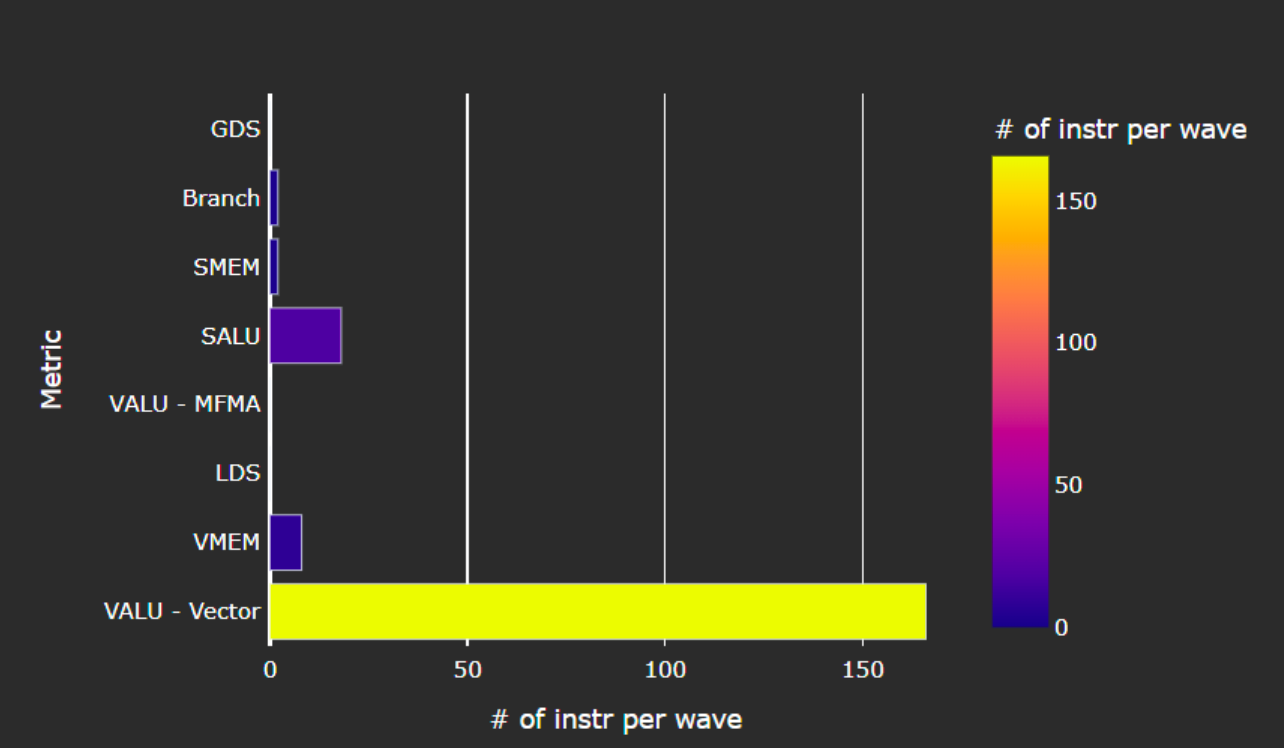
\includegraphics[width=0.5\linewidth]{Appendici/InstructionMixPanel.png}
        \caption{綜合指令面板 (Instruction Mix Panel) 顯示每個 wavefront 中每種指令類型的平均數量}
        \label{fig:instruction-mix-panel}
    \end{subfigure}

    \begin{subfigure}[b]{\textwidth}
        \centering
        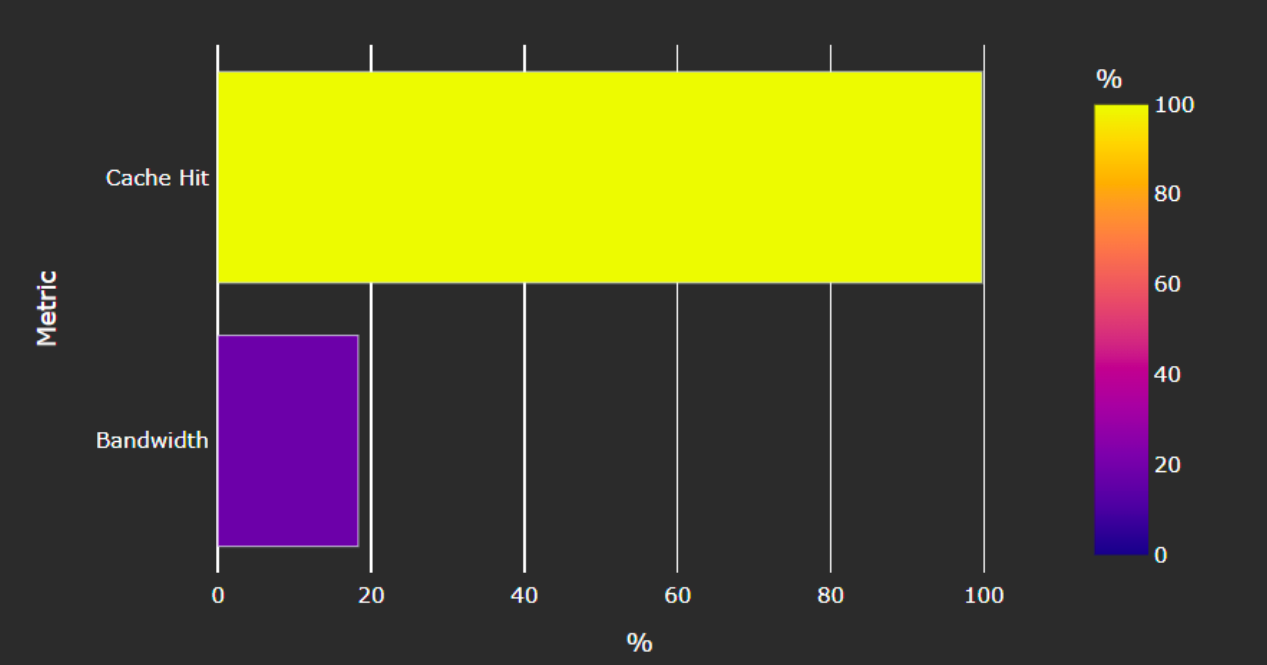
\includegraphics[width=0.5\linewidth]{Appendici/L1CachePanel.png}
        \caption{L1 快取面板 (L1 Cache panel) 顯示快取命中率和頻寬使用率。}
        \label{fig:l1-cache-panel}
    \end{subfigure}

    \caption{Omniperf 中基於 Grafana 的分析工具所提供的範例視圖}
    
\end{figure}

\section{總結}
在本附錄章節中,我們介紹了兩個進階的效能分析工具:1) Omnitrace 與 2) Omniperf。這些工具擴展了內建 ROCm 工具(rocTracer 和 rocProfiler)的功能,提供了捕捉程式執行追蹤和效能指標的能力。Omnitrace 和 Omniperf 提供了額外的分析和視覺化選擇,簡化了優化程式效能的過程。
